\appendix
\chapter{Appendix A: Statistics}
\addcontentsline{toc}{chapter}{Appendix B: Performance of other models..?}
\section{Statistics}
% remove comment if you wish to add Appendix to contentsline.
%\addcontentsline{toc}{chapter}{Appendix A: How to download ERA5 data}

%%% CORRELATION
\begin{figure}[ht]
    \centering
    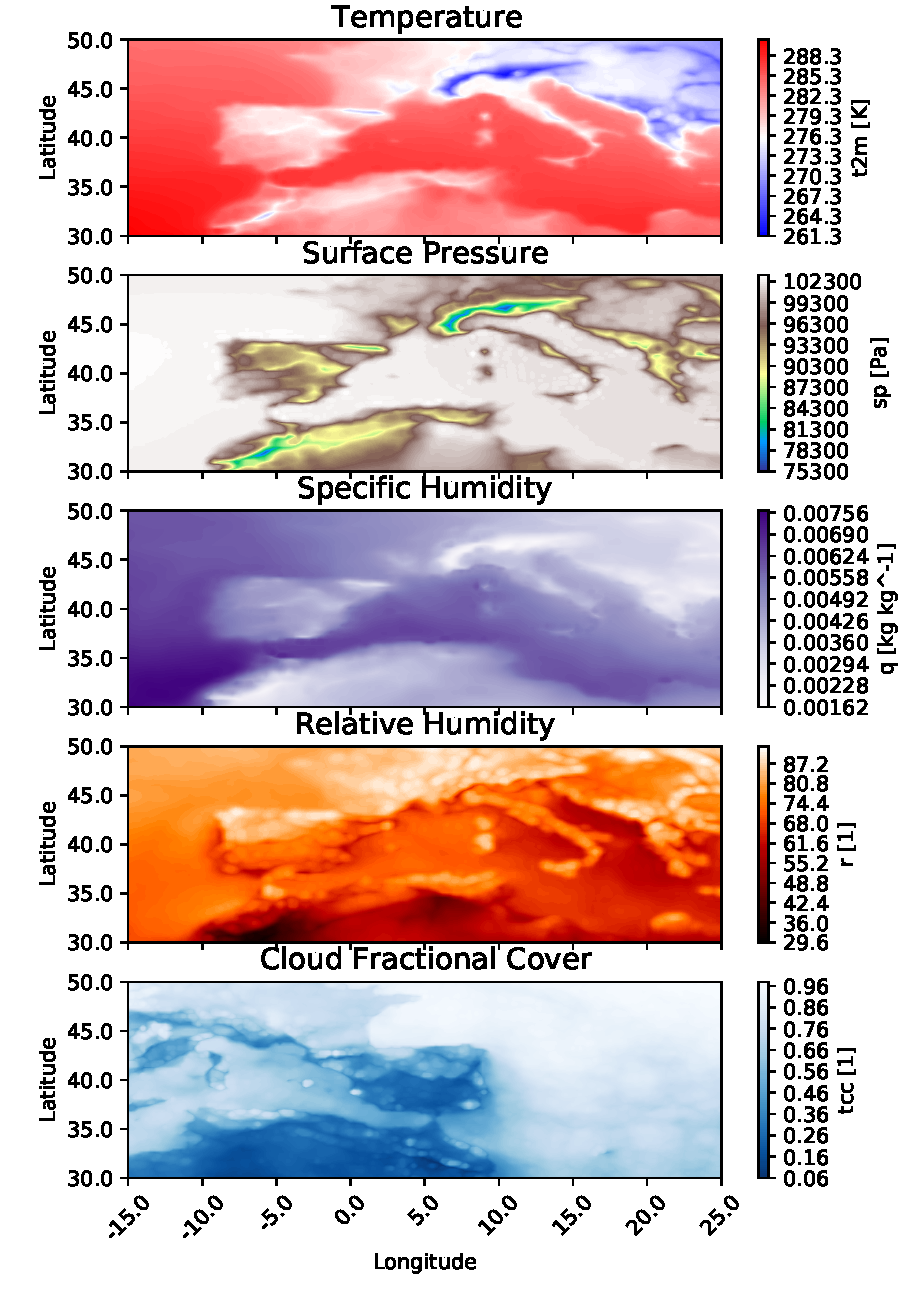
\includegraphics{python_figs/contour_temporally_averaged.pdf}
    \caption{Contour plot showing the correlation between enviornmental variables and cloud fractional cover. }
    \label{fig:correlation_tcc_vs_envio}
\end{figure}

%%% BAR PLOT GLOBAL STATISTICS
\begin{figure}[ht]
    \centering
    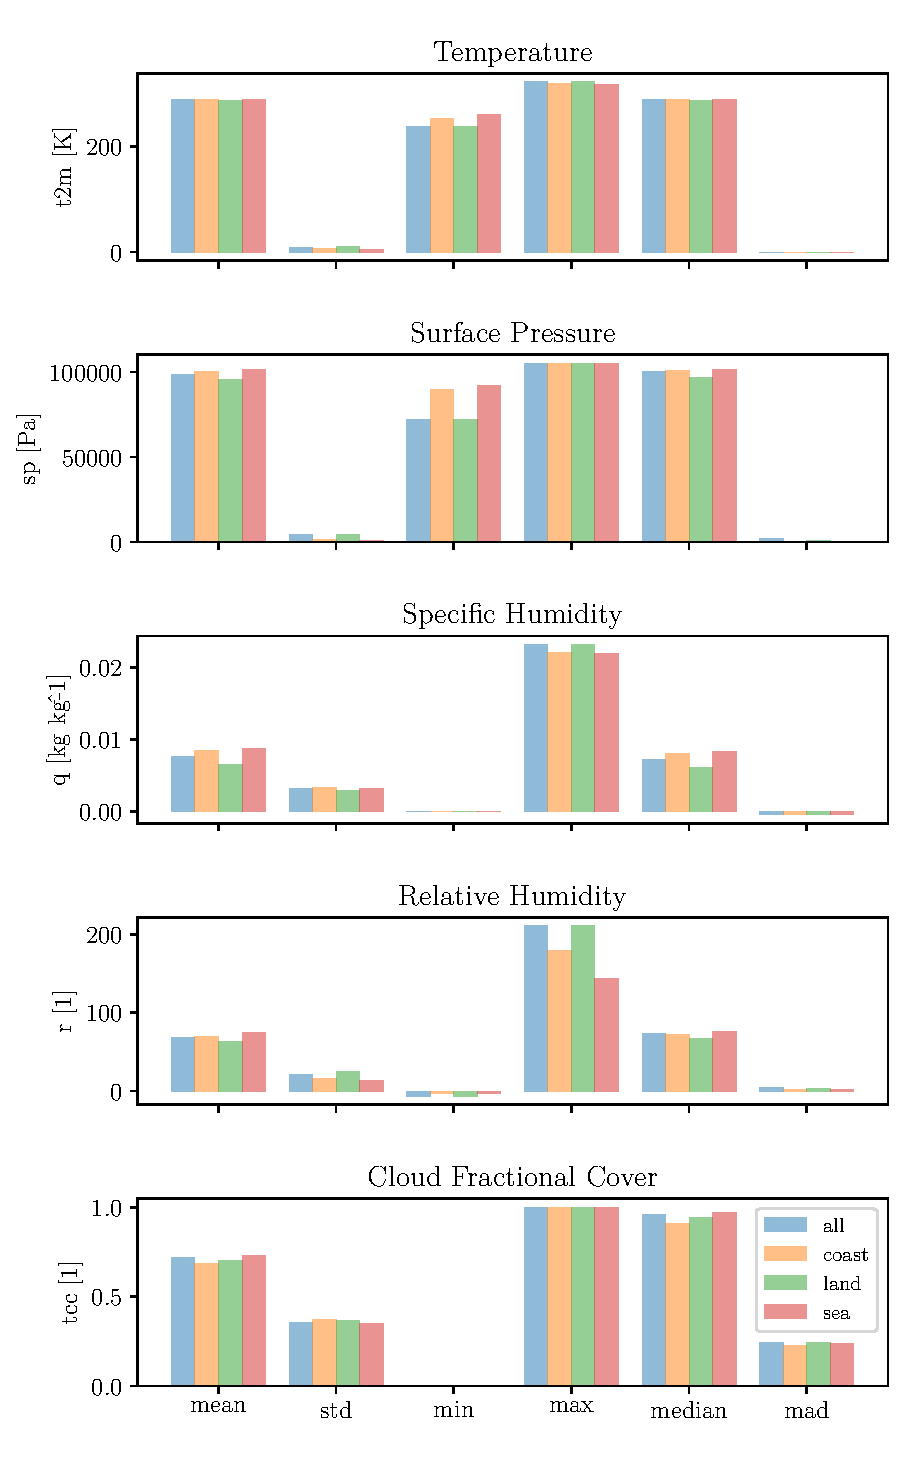
\includegraphics{python_figs/bar_plot_global_statistics.pdf}
    \caption{Bar plot showing global statistics for different filters.}
    \label{fig:bar_plot_global_stats}
\end{figure}

\subsection{Alternative 1}

%%% ALL LOCAL STATISTICS FOR VARIABLES 
%% TEMPERATURE
\begin{figure}[ht]
    \centering
    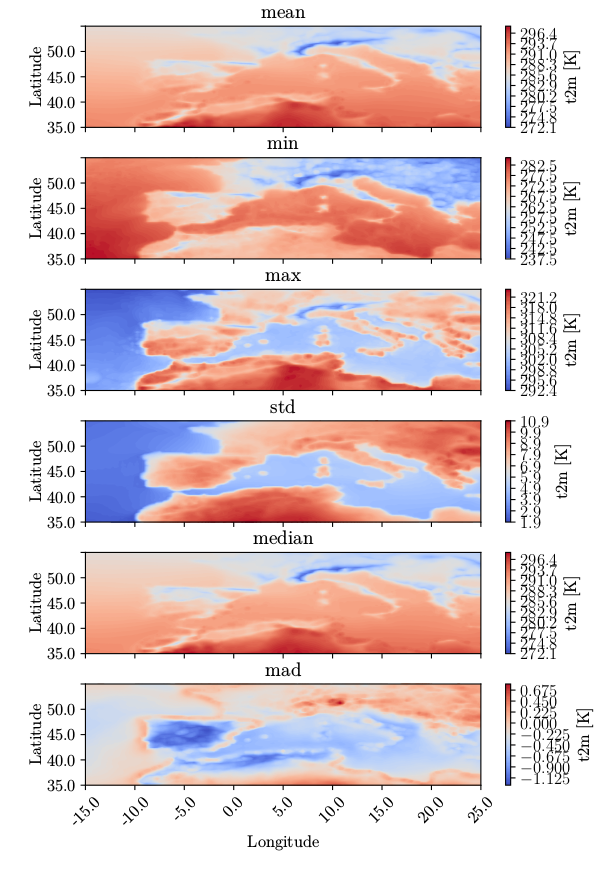
\includegraphics{python_figs/all_stat_variable_t2m.png}
    \caption{Contour plot showing the local (pixel) statistics for temperature.}
    \label{fig:all_stats_t2m}
\end{figure}

%% SURFACE PRESSURE 
\begin{figure}[ht]
    \centering
    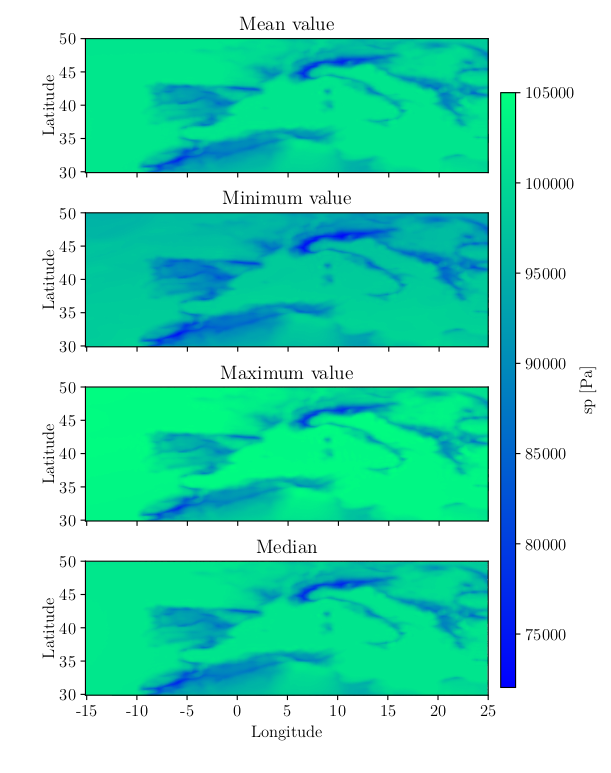
\includegraphics{python_figs/all_stat_variable_sp.png}
    \caption{Contour plot showing the local (pixel) statistics for surface pressure.}
    \label{fig:all_stats_sp}
\end{figure}

%% RELATIVE HUMIDITY 
\begin{figure}[ht]
    \centering
    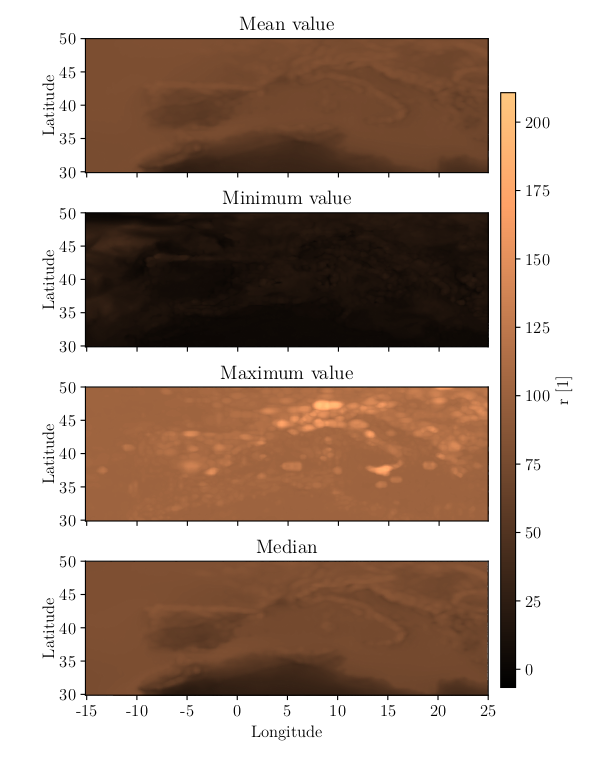
\includegraphics{python_figs/all_stat_variable_r.png}
    \caption{Contour plot showing the local (pixel) statistics for relative humidity.}
    \label{fig:all_stats_r}
\end{figure}


%% SPECIFIC HUMIDITY 
\begin{figure}[ht]
    \centering
    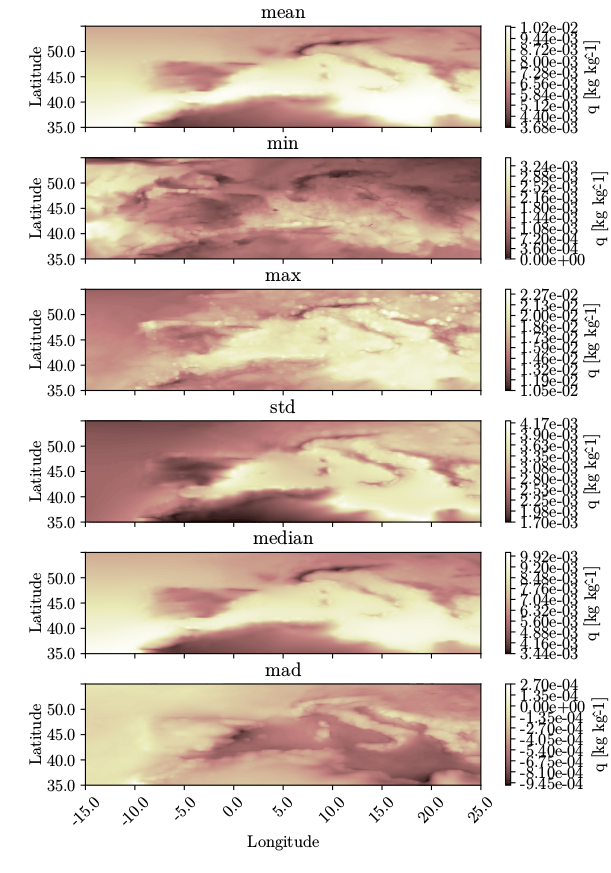
\includegraphics{python_figs/all_stat_variable_q.png}
    \caption{Contour plot showing the local (pixel) statistics for spesific humidity.}
    \label{fig:all_stats_q}
\end{figure}


%% CLOUD FRACTIONAL COVER
\begin{figure}[ht]
    \centering
    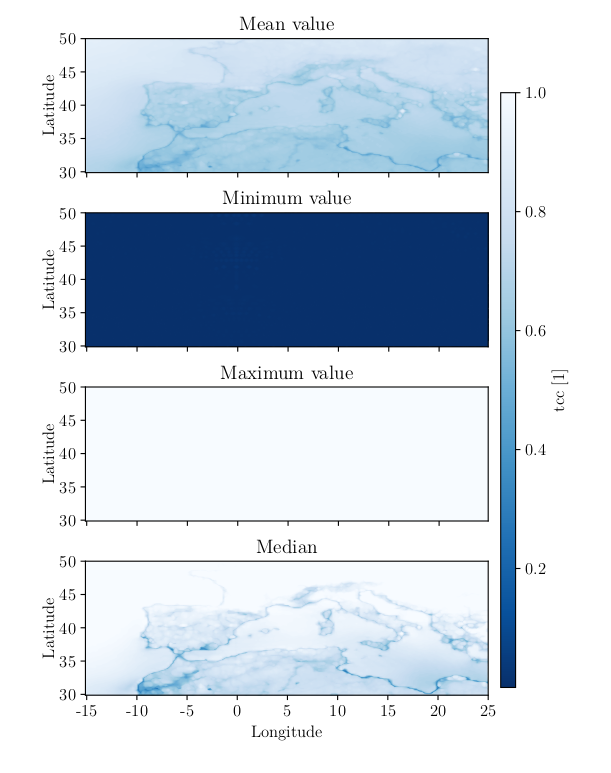
\includegraphics{python_figs/all_stat_variable_tcc.png}
    \caption{Contour plot showing the local (pixel) statistics for cloud fractional cover.}
    \label{fig:all_stats_tcc}
\end{figure}

%%%%%% CONTOUR PLOTS SHOWING 
\subsection{Alternative 2 - skal snu skydekket}
%%%% STD
\begin{figure}[ht]
    \centering
    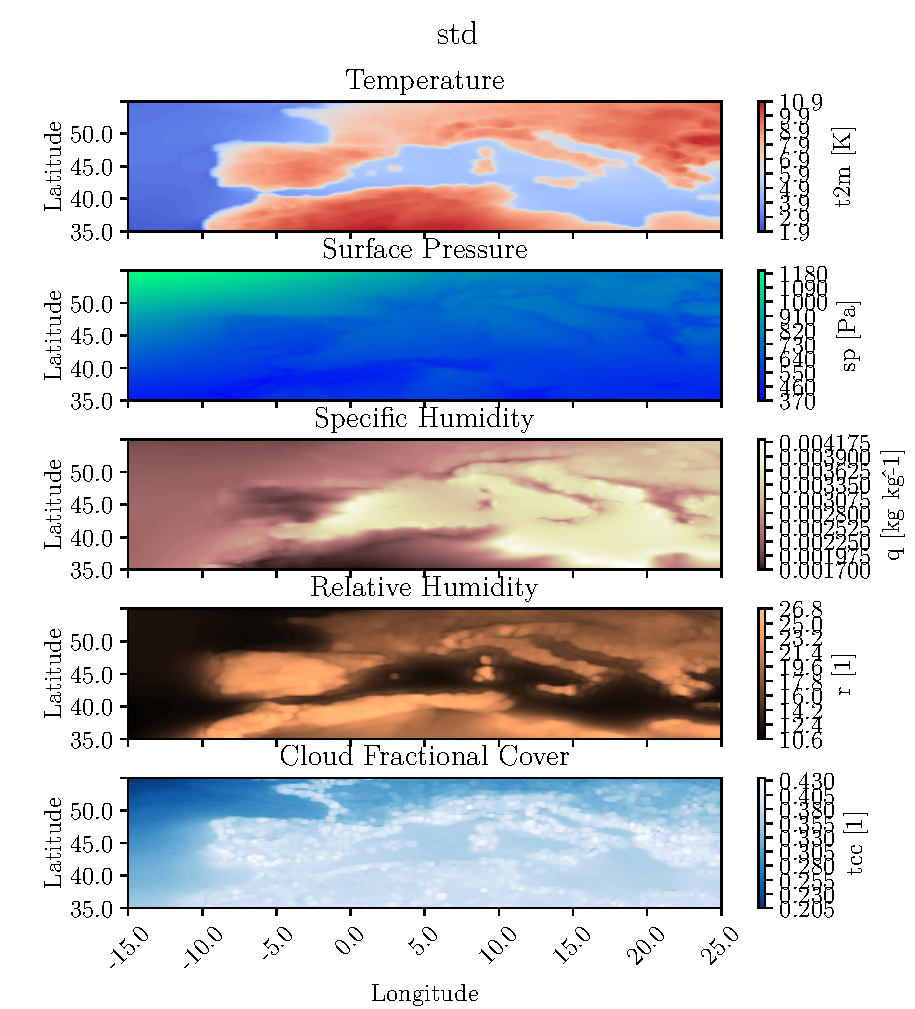
\includegraphics{python_figs/contourplot_all_variables_std.pdf}
    \caption{Contour plot showing the local (pixel) standard deviation of all variables.}
    \label{fig:contour_std_all_vars}
\end{figure}

%%%% MIN
\begin{figure}[ht]
    \centering
    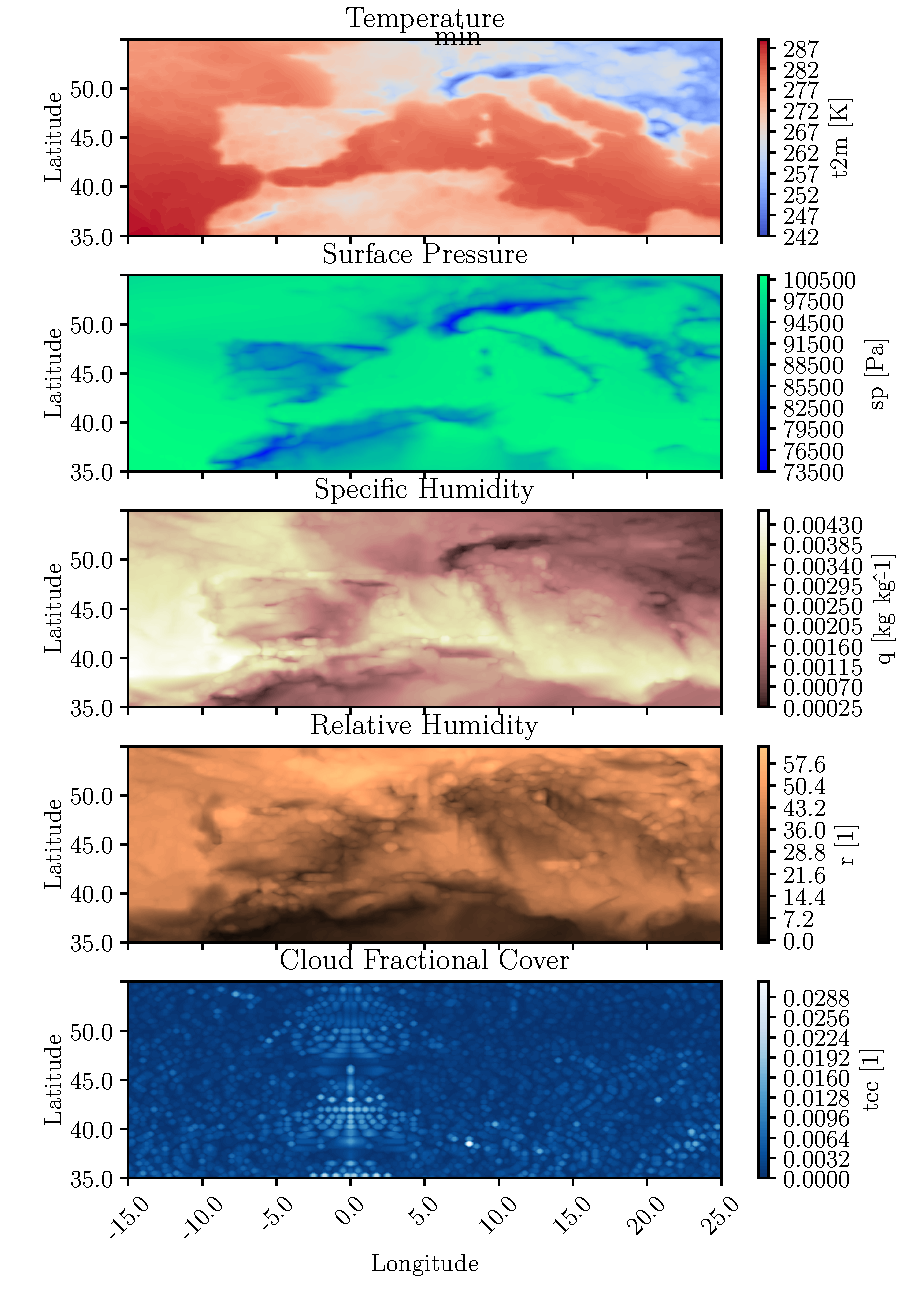
\includegraphics{python_figs/contourplot_all_variables_min.pdf}
    \caption{Contour plot showing the local (pixel) minimum of all variables.}
    \label{fig:contour_min_all_vars}
\end{figure}


%%%% MAX
\begin{figure}[ht]
    \centering
    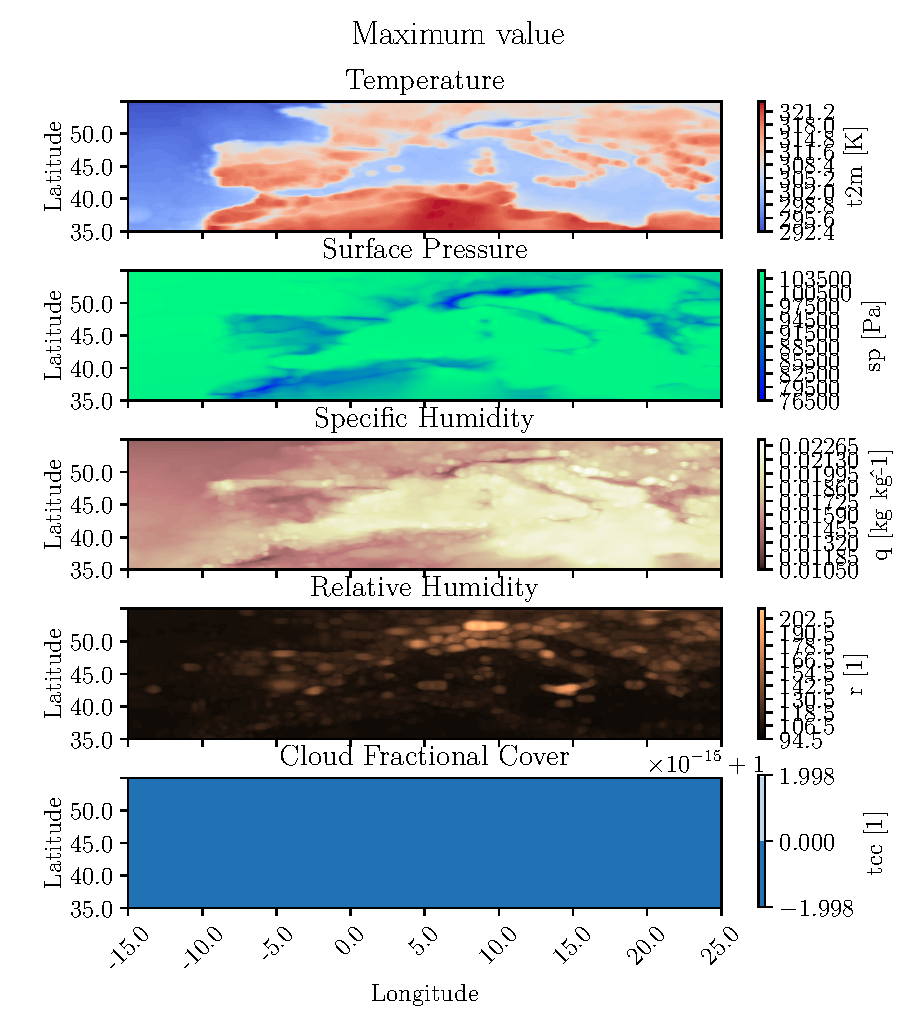
\includegraphics{python_figs/contourplot_all_variables_max.pdf}
    \caption{Contour plot showing the local (pixel) max of all variables.}
    \label{fig:contour_max_all_vars}
\end{figure}


%%%% MAD
\begin{figure}[ht]
    \centering
    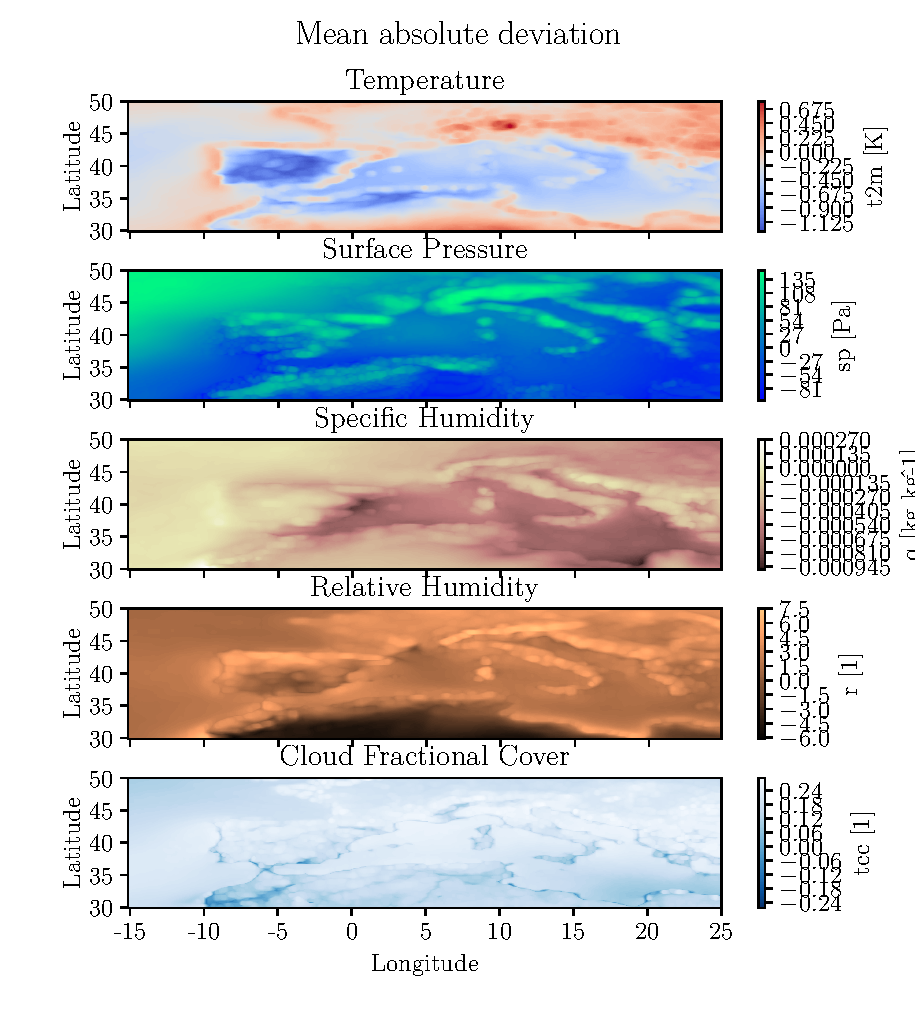
\includegraphics{python_figs/contourplot_all_variables_mad.pdf}
    \caption{NOT generated yet! Contour plot showing the local (pixel) mad of all variables.}
    \label{fig:contour_mad_all_vars}
\end{figure}


%%%% MEAN
\begin{figure}[ht]
    \centering
    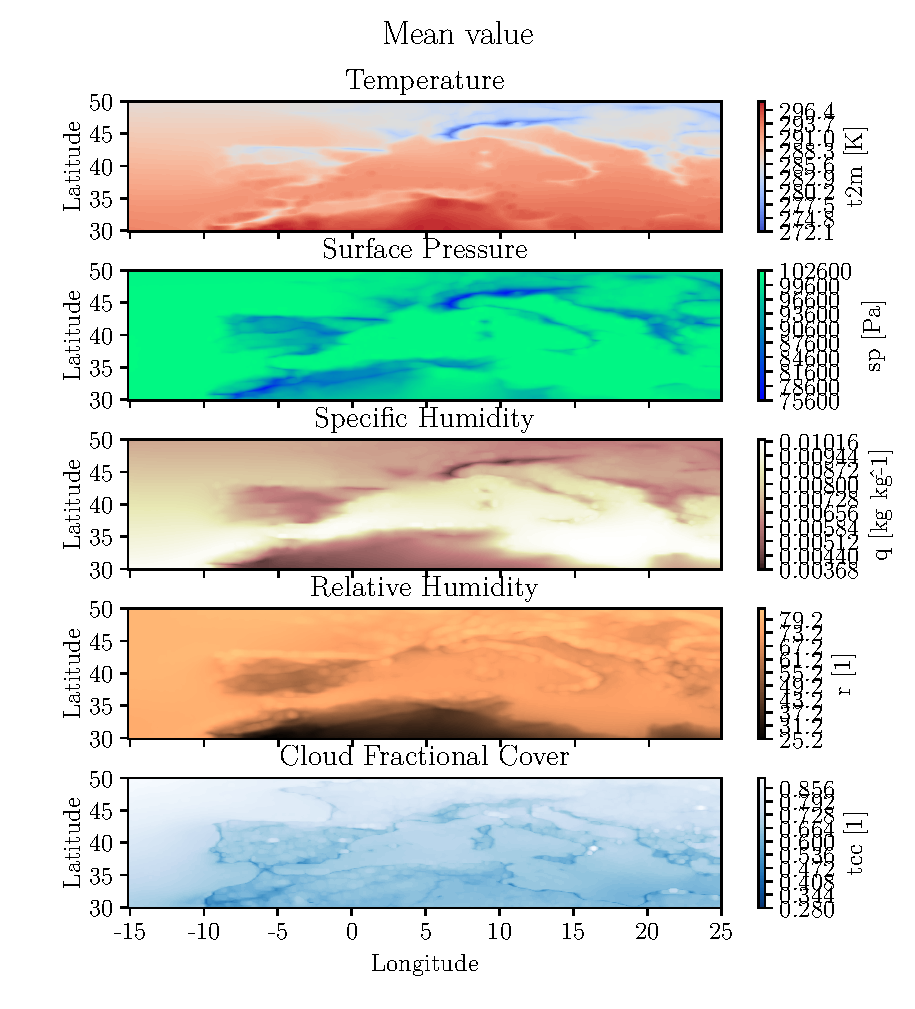
\includegraphics{python_figs/contourplot_all_variables_mean.pdf}
    \caption{Contour plot showing the local (p ixel) mean of all variables.}
    \label{fig:contour_mean_all_vars}
\end{figure}


%%%% MEDIAN
\begin{figure}[ht]
    \centering
    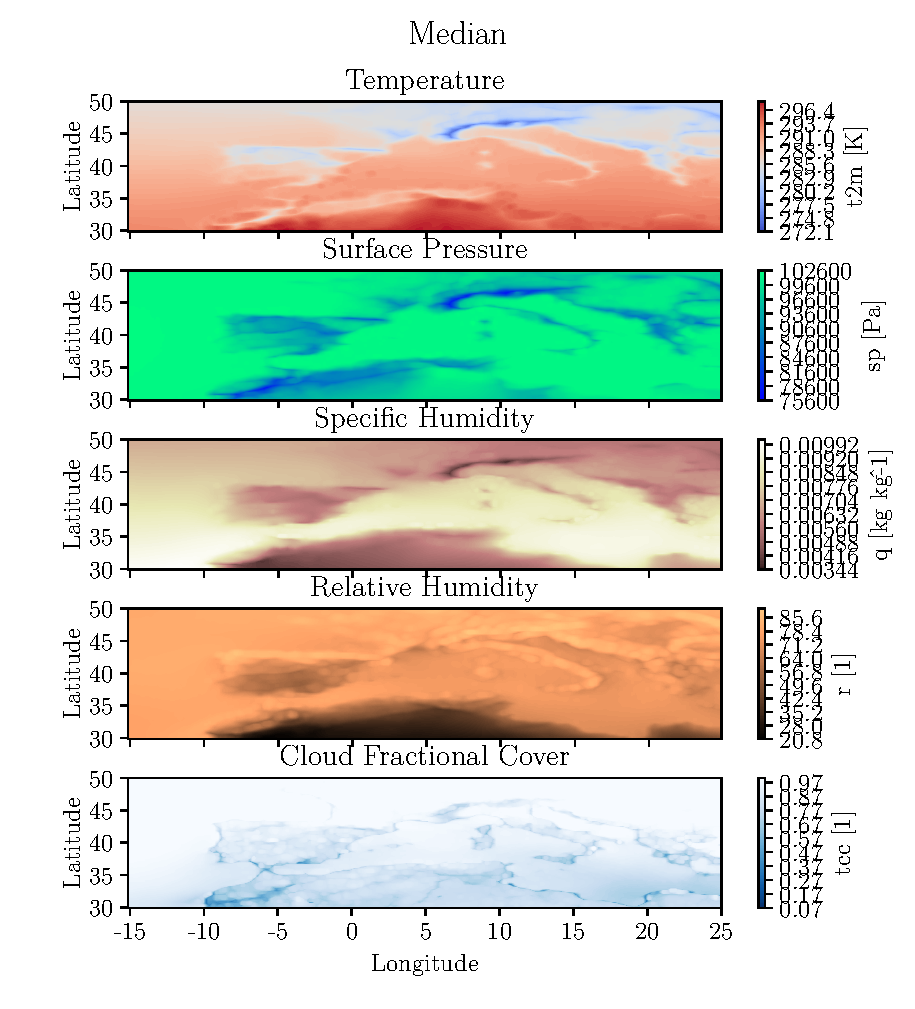
\includegraphics{python_figs/contourplot_all_variables_median.pdf}
    \caption{Contour plot showing the local (pixel) median of all variables.}
    \label{fig:contour_mean_all_vars}
\end{figure}




\cleardoublepage

\chapter{Performance of other models..?}
\addcontentsline{toc}{chapter}{Appendix B: Performance of other models..?}

%%%% TARGET PREDICITON HORIZONTAL
\begin{figure}[ht]
    \centering
    \includegraphics{python_figs/target_prediction_plot_horizonal.pdf}
    \caption{Comparison target and predicted cloud fractinal cover.}
    \label{fig:target_predict_horizontal}
\end{figure}

%%%% TARGET PREDICITON HORIZONTAL
\begin{figure}[ht]
    \centering
    \includegraphics{python_figs/target_prediction_plot_vertical.pdf}
    \caption{Comparison target and predicted vertical cloud fractional cover.}
    \label{fig:target_predict_vertical}
\end{figure}

%%%%%%%%%% Dummy model performance plot
\begin{figure}[ht]
    \centering
    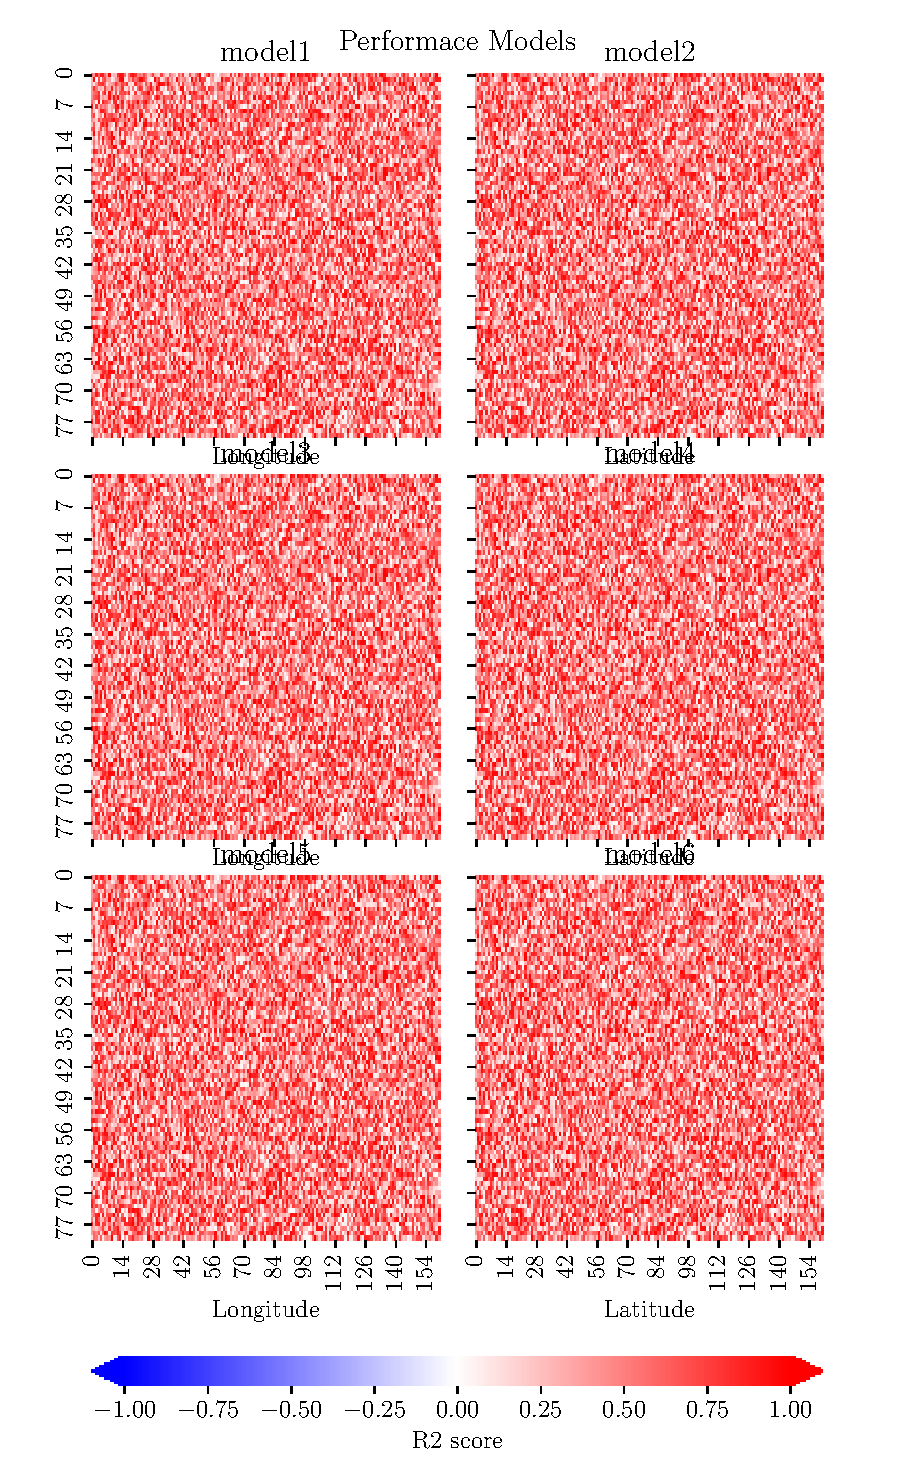
\includegraphics{python_figs/dummy_model_performace_plot.pdf}
    \caption{Dummy performance plot.}
    \label{fig:dummy_performace_plot}
\end{figure}

%%%%%%%%%% Dummy model performance plot - CROSSVALIDATION
\begin{figure}[ht]
    \centering
    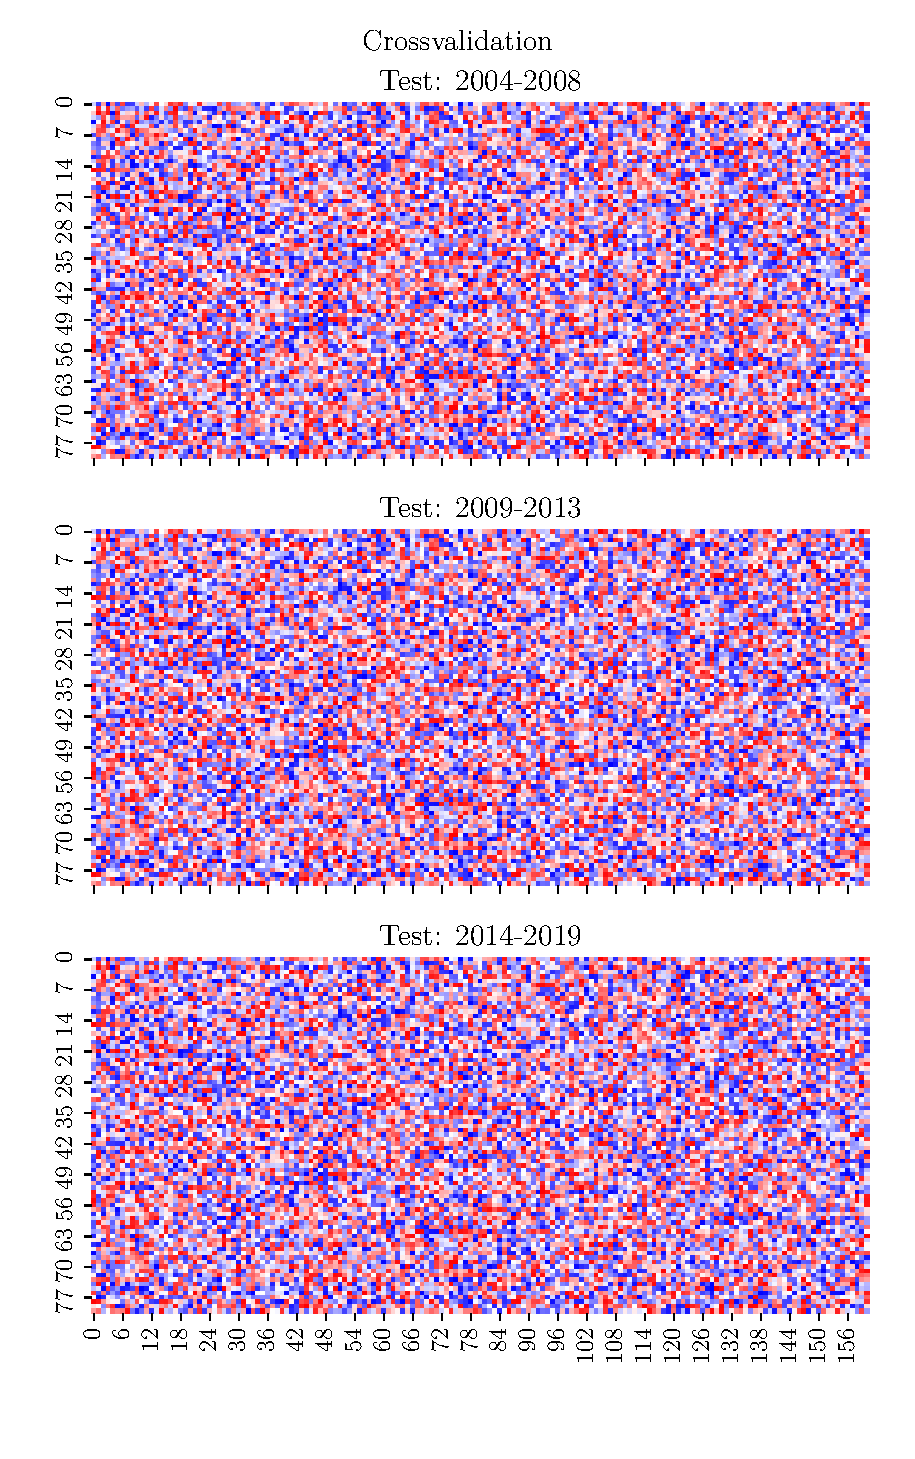
\includegraphics{python_figs/dummy_model_performace_cross_validation_plot.pdf}
    \caption{Dummy performance plot - crossvalidation edition.}
    \label{fig:dummy_performace_plot_crossvalidation}
\end{figure}


\cleardoublepage
